\documentclass[11pt,letterpaper]{article}
\usepackage[lmargin=2.2in,rmargin=0.7in,tmargin=1.0in,bmargin=1.0in]{geometry}
\usepackage{notes}
\begin{document}

\begin{center}
\Large\textbf{DAY 34 -- Repeated Eigenvalues: Stars, Degenerate Nodes}\\
\normalsize (Section 4.4.3)
\end{center}


%-------------------------------------------------------------
\section{Repeated Eigenvalues}

\subsection{The Last Case}
In the past few lectures, we have been studying different cases for solutions to the system
$$
    \mathbf{x}' = A \mathbf{x}.
$$
We have the general solution when the eigenvalues are 
\begin{enumerate}
    \item[a)] real and distinct $\lambda_1\ne \lambda_2$, and
    \item[b)] nonreal $\lambda_{1,2}=\alpha \pm i\beta$ with $\beta\ne0$.
\end{enumerate}
Today, we will study the last case: when the eigenvalue is repeated, $\lambda_1=\lambda_2$. This last case separates into two subcases. To illustrate this point, we will examine two matrices with the same characteristic polynomial.

\subsection{Compare the Matrices}
Consider the two matrices
$$
A = \begin{pmatrix}
    2 & 0\\
    0 & 2
\end{pmatrix} \qquad\text{and}\qquad B = \begin{pmatrix}
    3 &1\\
    -1 & 1
\end{pmatrix}.
$$
Let's find the eigenvalues of both matrices:
\begin{align*}
    \det(A-\lambda I)&=0 & \det(B-\lambda I)&=0\\
    \begin{vmatrix}2-\lambda & 0\\ 0&2-\lambda \end{vmatrix} &=0 & \begin{vmatrix} 3-\lambda& 1\\ -1&1-\lambda\end{vmatrix}&=0\\
    (\lambda-2)^2&=0 & \lambda^2-4\lambda+4&=0\\
    & & (\lambda-2)^2&=0
\end{align*}
Both matrices have the repeated eigenvalue $\lambda=2$. How many independent eigenvectors can we find for each matrix? Substitute $\lambda=2$ into the two systems below.
\begin{align*}
    (A-\lambda I)\mathbf{v} &= \mathbf{0}   & (B-\lambda I)\mathbf{w} &= \mathbf{0} \\
    \begin{pmatrix}0 & 0\\ 0&0 \end{pmatrix}\begin{pmatrix}
        v_1\\v_2
    \end{pmatrix} &=\begin{pmatrix}
        0\\0
    \end{pmatrix} & \begin{pmatrix} 1& 1\\ -1&-1\end{pmatrix}\begin{pmatrix}
        w_1\\w_2
    \end{pmatrix}&=\begin{pmatrix}
        0\\0
    \end{pmatrix}
\end{align*}
For $A$, the equations impose no restrictions. Every nonzero vector is an eigenvector, so we can choose two independent ones. For $B$, the equation $w_1+w_2=0$ leaves one free variable. Every eigenvector lies on the line $w_2=-w_1$. We can choose
\begin{align*}
    \mathbf{v}_1 &= \begin{pmatrix}
        1\\0
    \end{pmatrix}, \mathbf{v}_2=\begin{pmatrix}
        0\\1
    \end{pmatrix}, &
    \mathbf{w}&= \begin{pmatrix}
        1\\-1
    \end{pmatrix}.
\end{align*}
When a matrix has repeated eigenvalues, there are two subcases: 
\begin{itemize}
    \item[a)] the matrix has two independent eigenvectors, or
    \item[b)] the matrix has only one independent eigenvector.
\end{itemize}

\subsection{Goal}
We will study the two subcases of when $A$ has repeated eigenvalues.
\begin{enumerate}
    \item \textbf{Case 1}: $A$ has two eigenvectors that are not constant multiples of each other $\mathbf{v}_1\ne c\mathbf{v}_2$. In this case, the general solution is as usual:
     $$\mathbf{x}(t) = c_1 \mathbf{v}_1 e^{\lambda t} + c_2 \mathbf{v}_2 e^{\lambda t}.$$ 
     
    \item \textbf{Case 2}: $A$ has only one independent eigenvector $\mathbf{v}$. In this case, the general solution needs a slight modification.
\end{enumerate}


%-------------------------------------------------------------

\section{Case 1: Independent Eigenvectors}

\subsection{Same $\lambda$ but Different Eigenvectors}
If $\lambda$ is an eigenvalue of $A$ then its eigenvector $\mathbf{v}$ satisfies 
$$
(A-\lambda I)\mathbf{v} = \mathbf{0}.
$$
Suppose the repeated eigenvalue $\lambda$ has two independent eigenvectors. Every vector in the plane is a linear combination of those two vectors, so $A$ multiplies every vector by $\lambda$. Thus
\[
A=\lambda I=\begin{bmatrix}\lambda&0\\0&\lambda\end{bmatrix}.
\]
For $\lambda\ne0$, this gives a star node. If $\lambda=0$, then $A=0$ and every point is an equilibrium.
\begin{example}[1]{
Find the general solution to 
\[
\mathbf{x}'=\begin{bmatrix}3&0\\0&3\end{bmatrix} \mathbf{x}.
\]
}
\paragraph{Step 1. Find the eigenvalues.}
$$
0 = \det(\lambda I - A) = \begin{vmatrix}
    \lambda-3 & 0 \\
    0 & \lambda-3
\end{vmatrix} = (\lambda-3)^2 \implies \lambda=3.
$$
\paragraph{Step 2. Find the eigenvectors.}
\begin{align*}
    (A-\lambda I)\mathbf{v}_1&=\mathbf{0}\\
    \left(\begin{bmatrix}
        3 & 0\\ 0 &3
    \end{bmatrix}-\begin{bmatrix}
        3 & 0\\ 0 & 3
    \end{bmatrix}\right)\mathbf{v}_1&=\mathbf{0}\\
     \begin{bmatrix}
        0 & 0\\ 0 &0
    \end{bmatrix}\mathbf{v}_1&=\mathbf{0}
\end{align*}
Every nonzero vector satisfies this equation. To get two independent solutions, choose two independent eigenvectors. The coordinate vectors are convenient:
\[
\mathbf{v}_1=\begin{bmatrix}1\\0\end{bmatrix},
\qquad
\mathbf{v}_2=\begin{bmatrix}0\\1\end{bmatrix}.
\]
\paragraph{Step 3. Write the general solution.}
\begin{align*}
\mathbf{x}(t) &= c_1 \mathbf{v}_1 e^{\lambda_1 t} + c_2 \mathbf{v}_2 e^{\lambda_2 t}\\
&=c_1 \begin{bmatrix}
    1\\0
\end{bmatrix} e^{3t} + c_2 \begin{bmatrix}
    0\\1
\end{bmatrix}e^{3t}.
\end{align*}
There is no need to deviate from our usual formula since the eigenvectors are independent.
\end{example}

%-------------------------------------------------------------
\section{The Star Node}

\subsection{Solution Curves}
Let's sketch a few solution curves for 
$$
\mathbf{x}=c_1 \begin{bmatrix}
    1\\0
\end{bmatrix} e^{3t} + c_2 \begin{bmatrix}
    0\\1
\end{bmatrix}e^{3t}.
$$
If $c_1=0$ and $c_2\ne0$, the trajectory lies on one of the two $y$-axis rays. If $c_1\ne0$, then
\[
x=c_1e^{3t},\qquad y=c_2e^{3t}
\qquad\Longrightarrow\qquad y=\frac{c_2}{c_1}x.
\]
The factor $e^{3t}$ is positive, so each nonconstant trajectory follows one ray and points away from the origin. The origin itself is an equilibrium. Drawing several rays gives the star shape below.
\begin{figure}[H]
\centering
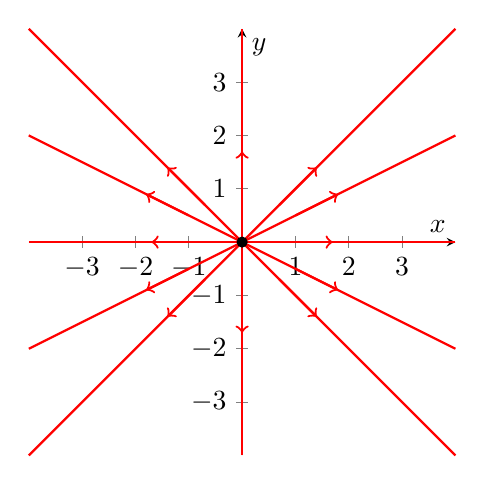
\begin{tikzpicture}
\begin{axis}[
    width=7cm,
    height=7cm,
    axis lines=middle,
    xmin=-4, xmax=4,
    ymin=-4, ymax=4,
    xtick={-3,-2,-1,1,2,3},
    ytick={-3,-2,-1,1,2,3},
    xlabel={$x$},
    ylabel={$y$},
    axis equal image,
    clip=false
]

% solution curves (straight lines through the origin)
\addplot[red,thick,domain=-4:4] {0};
\addplot[red,thick,domain=-4:4] {x};
\addplot[red,thick,domain=-4:4] {-x};
\addplot[red,thick,domain=-4:4] {0.5*x};
\addplot[red,thick,domain=-4:4] {-0.5*x};

% y-axis orbit
\addplot[red,thick,domain=-4:4,samples=2] coordinates {(0,-4) (0,4)};

% arrows pointing away from the origin
\draw[red,->,thick] (axis cs:0.9,0) -- (axis cs:1.7,0);
\draw[red,->,thick] (axis cs:-0.9,0) -- (axis cs:-1.7,0);
\draw[red,->,thick] (axis cs:0,0.9) -- (axis cs:0,1.7);
\draw[red,->,thick] (axis cs:0,-0.9) -- (axis cs:0,-1.7);
\draw[red,->,thick] (axis cs:0.7,0.7) -- (axis cs:1.4,1.4);
\draw[red,->,thick] (axis cs:-0.7,-0.7) -- (axis cs:-1.4,-1.4);
\draw[red,->,thick] (axis cs:0.7,-0.7) -- (axis cs:1.4,-1.4);
\draw[red,->,thick] (axis cs:-0.7,0.7) -- (axis cs:-1.4,1.4);
\draw[red,->,thick] (axis cs:1.0,0.5) -- (axis cs:1.8,0.9);
\draw[red,->,thick] (axis cs:-1.0,-0.5) -- (axis cs:-1.8,-0.9);
\draw[red,->,thick] (axis cs:1.0,-0.5) -- (axis cs:1.8,-0.9);
\draw[red,->,thick] (axis cs:-1.0,0.5) -- (axis cs:-1.8,0.9);

% origin
\addplot[only marks,mark=*,mark size=1.8pt] coordinates {(0,0)};

\end{axis}
\end{tikzpicture}
\caption{An unstable star.}
\end{figure}

\subsection{Classification}
Whenever you have a linear system of the form 
$$
\mathbf{x}' = \begin{bmatrix}
    a & 0 \\
    0 & a
\end{bmatrix}\mathbf{x},
$$
with $a\ne0$, the equilibrium point is called a \textbf{star node}. This system has only one eigenvalue $\lambda=a$ (you should verify this). The equilibrium is located at the origin, $\mathbf{x}^* = \mathbf{0}$. The stability of the equilibrium depends on the sign of $a$. If $a<0$, then we have a \textbf{stable star}. If $a>0$, then we have an \textbf{unstable star.}

\begin{example}[2]{
Sketch the phase portrait and classify the equilibrium for the system
\[
\mathbf{x}' = \begin{bmatrix}
    -2 & 0\\
    0 & -2
\end{bmatrix}\mathbf{x}.
\]
}
This is a star node with an eigenvalue $\lambda=-2$. Every nonconstant trajectory lies on a ray. Since $\lambda<0$, draw an arrow toward the origin on each ray. For the classification, we say 
$$
\boxed{\text{(0,0) is a stable star.}}
$$
\begin{figure}[H]
\centering
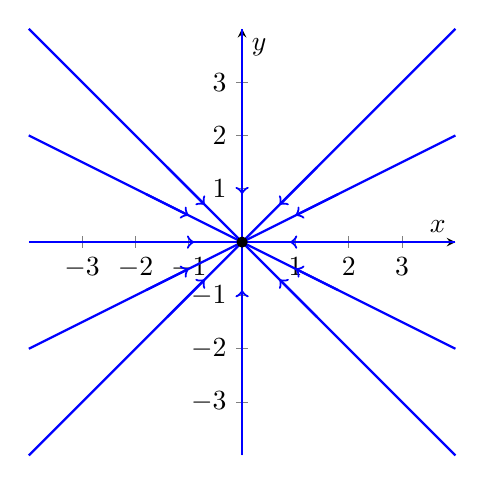
\begin{tikzpicture}
\begin{axis}[
    width=7cm,
    height=7cm,
    axis lines=middle,
    xmin=-4, xmax=4,
    ymin=-4, ymax=4,
    xtick={-3,-2,-1,1,2,3},
    ytick={-3,-2,-1,1,2,3},
    xlabel={$x$},
    ylabel={$y$},
    axis equal image,
    clip=false
]

% solution curves (straight lines through the origin)
\addplot[blue,thick,domain=-4:4] {0};
\addplot[blue,thick,domain=-4:4] {x};
\addplot[blue,thick,domain=-4:4] {-x};
\addplot[blue,thick,domain=-4:4] {0.5*x};
\addplot[blue,thick,domain=-4:4] {-0.5*x};

% y-axis orbit
\addplot[blue,thick,domain=-4:4,samples=2] coordinates {(0,-4) (0,4)};

% arrows pointing away from the origin
\draw[blue,<-,thick] (axis cs:0.9,0) -- (axis cs:1.7,0);
\draw[blue,<-,thick] (axis cs:-0.9,0) -- (axis cs:-1.7,0);
\draw[blue,<-,thick] (axis cs:0,0.9) -- (axis cs:0,1.7);
\draw[blue,<-,thick] (axis cs:0,-0.9) -- (axis cs:0,-1.7);
\draw[blue,<-,thick] (axis cs:0.7,0.7) -- (axis cs:1.4,1.4);
\draw[blue,<-,thick] (axis cs:-0.7,-0.7) -- (axis cs:-1.4,-1.4);
\draw[blue,<-,thick] (axis cs:0.7,-0.7) -- (axis cs:1.4,-1.4);
\draw[blue,<-,thick] (axis cs:-0.7,0.7) -- (axis cs:-1.4,1.4);
\draw[blue,<-,thick] (axis cs:1.0,0.5) -- (axis cs:1.8,0.9);
\draw[blue,<-,thick] (axis cs:-1.0,-0.5) -- (axis cs:-1.8,-0.9);
\draw[blue,<-,thick] (axis cs:1.0,-0.5) -- (axis cs:1.8,-0.9);
\draw[blue,<-,thick] (axis cs:-1.0,0.5) -- (axis cs:-1.8,0.9);

% origin
\addplot[only marks,mark=*,mark size=1.8pt] coordinates {(0,0)};

\end{axis}
\end{tikzpicture}
\caption{A stable star.}
\end{figure}
\end{example}

%-------------------------------------------------------------
\section{Case 2: One Independent Eigenvector}

\subsection{Deficient Matrices}
Consider the matrix 
\[
A=\begin{bmatrix}4&2\\[2pt]0&4\end{bmatrix}.
\]
The eigenvalues are $\lambda_1=\lambda_2=4$. We can calculate its eigenvector
\begin{align*}
    (A-\lambda I)\mathbf{v}&=\mathbf{0}\\
     \begin{bmatrix}
        0 & 2\\ 0 &0
    \end{bmatrix}\mathbf{v}&=\mathbf{0}
\end{align*}
The only restriction is $v_2=0$. Choose $v_1=1$ to obtain $\mathbf{v}=(1,0)^T$. Every eigenvector is a nonzero multiple of $\mathbf{v}$, so we have only one eigenvector direction. A $2\times2$ matrix with a repeated eigenvalue and only one independent eigenvector is called \textbf{deficient} (or \textbf{defective}).
\subsection{Generalized Eigenvector}
When $A$ is deficient, there exists a second independent vector called the \textit{generalized eigenvector}. The \textbf{generalized eigenvector} is a vector $\mathbf{w}$ satisfying
\[
(A-\lambda I)\mathbf{w}=\mathbf{v},
\]
where $(\lambda,\mathbf{v})$ is a known eigenpair for $A$. Just like $\mathbf{v}$, the generalized eigenvector is \textit{not} unique. In other words, there are infinitely many solutions to $(A-\lambda I)\mathbf{w}=\mathbf{v}$. On the other hand, if $A$ isn't deficient, then $(A-\lambda I)\mathbf{w}=\mathbf{v}$ won't have any solutions at all.

\begin{example}[3]{
Let's return to the previous example. Find a generalized eigenvector for the matrix  
\[
A=\begin{bmatrix}4&2\\[2pt]0&4\end{bmatrix}, \quad \lambda=4, \quad \mathbf{v}=\begin{bmatrix}
    1\\0
\end{bmatrix}
\]
}
To find the generalized eigenvector, we write out the system 
\begin{align*}    
(A-\lambda I)\mathbf{w}&=\mathbf{v},\\
\begin{bmatrix}0&2\\0&0\end{bmatrix}\mathbf{w}&=\begin{bmatrix}1\\[2pt]0\end{bmatrix}
\end{align*}
This system states that $w_2 = 1/2$ and $w_1$ is free. For simplicity, we can let $w_1=0$. Therefore, a generalized eigenvector of $A$ is 
$$
\mathbf{w} = \begin{bmatrix}
    0\\1/2
\end{bmatrix}.
$$
Choose a convenient value for the free variable, then use the equation to determine the other component.
\end{example}

\subsection{The Theorem}

\begin{theorem} If $\mathbf{w}$ is a generalized eigenvector of $A$ for the eigenpair $(\lambda,\mathbf{v})$ then 
$$
\mathbf{x}_2(t)=e^{\lambda t}(\mathbf{v}t+\mathbf{w})
$$
is a solution to the system $\mathbf{x}'=A\mathbf{x}$. 
\end{theorem}
\begin{proof}
By assumption, we have $(A-\lambda I)\mathbf{w}=\mathbf{v}$, which can be written as
$$
A\mathbf{w}=\lambda\mathbf{w}+\mathbf{v}.
$$
Let $\mathbf{x}_2(t)=e^{\lambda t}(\mathbf{v}t+\mathbf{w})$. Calculate the LHS 
\[
\text{LHS} = \mathbf{x}_2'(t)
= \lambda e^{\lambda t}(\mathbf{v}t+\mathbf{w}) + e^{\lambda t}\mathbf{v}
= e^{\lambda t}\big(\lambda\mathbf{v}t+\lambda\mathbf{w}+\mathbf{v}\big).
\]
Now compute the RHS:
\begin{align*}
\text{RHS} &= 
A\mathbf{x}_2(t)\\
&= A\!\left(e^{\lambda t}(\mathbf{v}t+\mathbf{w})\right)\\
&= e^{\lambda t}\big(A(\mathbf{v}t)+A\mathbf{w}\big)\\
&= e^{\lambda t}\big(\lambda\mathbf{v}t + (\lambda\mathbf{w}+\mathbf{v})\big)\\
&=\text{LHS}
\end{align*}
\end{proof}


\subsection{General Solution}
This theorem gives us a solution to $\mathbf{x}'=A\mathbf{x}$ given by the formula $\mathbf{x}_2(t)=e^{\lambda t}(\mathbf{v}t+\mathbf{w})$. This is independent from the first solution $\mathbf{x}_1(t)=\mathbf{v}e^{\lambda t}$. That means we may finally write the general solution to the system $\mathbf{x}' = A \mathbf{x}$ when $A$ is deficient:
\[
\boxed{
\mathbf{x}(t)=
c_1\mathbf{v}e^{\lambda t}
+c_2e^{\lambda t}(\mathbf{v}t+\mathbf{w}).
}
\]

\subsection{A Sign to Watch}
Either determinant convention gives the same eigenvalues. When using the formula above, always solve $(A-\lambda I)\mathbf{w}=\mathbf{v}$. Reversing the subtraction changes the sign of the right-hand side: $(\lambda I-A)\mathbf{w}=-\mathbf{v}$.
\begin{example}[4]{
Find the general solution to the \textit{deficient system}
\[
\mathbf{x}' = \begin{bmatrix}3&1\\-1&1\end{bmatrix}\mathbf{x}.
\]
}
\paragraph{Step 1. Find the eigenvalue.}
$$0=\det(A-\lambda I)=\begin{vmatrix}
    3-\lambda & 1\\-1 & 1-\lambda
\end{vmatrix}=3-4\lambda +\lambda^2 +1=(\lambda-2)^2 \implies \lambda=2$$
\paragraph{Step 2. Find the eigenvector.}
\[
(A-2I)\mathbf{v}=\mathbf{0}
\quad\Rightarrow\quad
\begin{bmatrix}1&1\\-1&-1\end{bmatrix}\mathbf{v}=\mathbf{0}
\ \Rightarrow\ 
\mathbf{v}=
\begin{bmatrix}1\\-1\end{bmatrix}.
\]
\paragraph{Step 3. Generalized eigenvector.}
\[
\begin{bmatrix}1&1\\-1&-1\end{bmatrix}\mathbf{w}=\begin{bmatrix}1\\-1\end{bmatrix}
\quad\implies\quad
\text{let } w_1=0,\text{then }w_2=1 
\quad\implies 
\mathbf{w}=\begin{bmatrix}0\\1\end{bmatrix}.
\]
\paragraph{Step 4. Apply the formula.}
\begin{align*}
    \mathbf{x}(t)&=c_1\mathbf{v}e^{\lambda t}+c_2e^{\lambda t}(\mathbf{v}t+\mathbf{w})\\
    &=c_1\begin{bmatrix}
        1\\-1
    \end{bmatrix}e^{2 t}+c_2e^{2 t}\left(\begin{bmatrix}
        1\\-1
    \end{bmatrix}t+\begin{bmatrix}
        0\\1
    \end{bmatrix}\right).
\end{align*}
\end{example}

%-------------------------------------------------------------
\section{Degenerate Node}

\subsection{Solution Curves for Deficient Systems}
Now let us analyze the solution
\[
\mathbf{x}(t)
=
c_1\mathbf{v}e^{\lambda t}
+
c_2 e^{\lambda t}\bigl(\mathbf{v}t+\mathbf{w}\bigr),
\]
where
\[
\mathbf{v}=\begin{bmatrix}1\\-1\end{bmatrix},
\qquad
\mathbf{w}=\begin{bmatrix}0\\1\end{bmatrix},
\qquad
\lambda=2.
\]
Factor the solution as
\[
\mathbf{x}(t)=e^{2t}\big[(c_1+c_2t)\mathbf{v}+c_2\mathbf{w}\big].
\]
If $c_2=0$, we get the two linear orbits on $y=-x$ and the equilibrium at the origin. Draw an outward arrow on each ray because $\lambda=2$.

If $c_2\ne0$, the coefficient of $\mathbf{v}$ grows in magnitude as $t\to\pm\infty$, while the coefficient of $\mathbf{w}$ stays constant inside the brackets. Near the origin ($t\to-\infty$), the trajectory is tangent to the eigenvector line. Far away ($t\to\infty$), its direction becomes parallel to the same line, along the opposite ray. For $c_2>0$, the trajectory starts near the $-\mathbf{v}$ ray and heads out in the $+\mathbf{v}$ direction. For $c_2<0$, the rays are reversed.

For this example, $x+y=c_2e^{2t}$ keeps its sign. Each curved trajectory therefore stays on its own side of the eigenvector line.
\subsection{Classification}
When the repeated eigenvalue satisfies $\lambda\ne0$ and $A$ is deficient, then the equilibrium is called a \textbf{degenerate node}. It is stable if $\lambda <0$ and unstable if $\lambda>0$. 

\subsection{Sketching the Phase Portrait}
a) Draw the eigenvector line and orient its two rays using the sign of $\lambda$.

b) Draw the velocity vector at a point off the line. In Example 4, $A(1,0)^T=(3,-1)^T$. At the positive $x$-axis the velocity points down, so the trajectories bend clockwise.

c) Sketch curves on both sides. Near the origin they are tangent to the eigenvector line. Far away they become parallel in direction to the opposite ray. Orient them to agree with the test vector.

\begin{center}
% The two systems are 2I +/- N, with N = B - 2I from Example 4.
\foreach \sign/\sense in {1/Clockwise,-1/Counterclockwise}{
\begin{tikzpicture}[scale=.48,>=Stealth]
\draw[->,gray] (-4.5,0)--(4.5,0) node[right] {$x$};
\draw[->,gray] (0,-4.5)--(0,4.5) node[above] {$y$};
\begin{scope}
\clip (-4,-4) rectangle (4,4);
\draw[red,thick] (-4,4)--(4,-4);
\foreach \k in {-1,1}{
    \draw[->,red,thick] (\k,-\k)--({1.8*\k},{-1.8*\k});
}
% The starting point is (a,b). Increasing t orients each curve.
\foreach \a/\b in {0/1,0/-1,0/3,0/-3,1/0,-1/0}{
    \draw[thick] plot[domain=-3:1.15,samples=95,variable=\t]
        ({exp(2*\t)*(\a+\sign*(\a+\b)*\t)},
         {exp(2*\t)*(\b-\sign*(\a+\b)*\t)});
    \draw[->,thick] plot[domain=-.12:.03,samples=12,variable=\t]
        ({exp(2*\t)*(\a+\sign*(\a+\b)*\t)},
         {exp(2*\t)*(\b-\sign*(\a+\b)*\t)});
}
\fill (0,0) circle (2pt);
\end{scope}
\node[below] at (0,-4.5) {\sense};
\end{tikzpicture}\hspace{.4em}
}

\small Left: Example 4. Right: the opposite shear with the same eigenvector line.
\end{center}
\begin{example}[5]{
Classify the equilibrium at the origin and sketch the phase portrait for
\[
\mathbf{x}'=
\begin{bmatrix}
-2 & 1\\
0 & -2
\end{bmatrix}\mathbf{x}.
\]
}
\paragraph{Step 1. Find the eigenvalue.}
\[
0=\det(\lambda I-A)
=
\begin{vmatrix}
\lambda+2 & -1\\
0 & \lambda+2
\end{vmatrix}
=(\lambda+2)^2\implies \lambda=-2.
\]
\paragraph{Step 2. Find the eigenvector.}
\[
(-2I-A)\mathbf{v}=\mathbf{0}
\implies
\begin{bmatrix}
0 & -1\\
0 & 0
\end{bmatrix}
\begin{bmatrix}
v_1\\v_2
\end{bmatrix}
=
\begin{bmatrix}
0\\0
\end{bmatrix}\implies 
\mathbf{v}=
\begin{bmatrix}
1\\0
\end{bmatrix}.
\]
\paragraph{Step 3. Write the general solution.}
Solve $(A+2I)\mathbf{w}=\mathbf{v}$. The first row gives $w_2=1$, so we can take $\mathbf{w}=(0,1)^T$. Thus
\[
\mathbf{x}(t)=e^{-2t}
\begin{pmatrix}c_1+c_2t\\c_2\end{pmatrix}.
\]
\paragraph{Step 4. Classify the equilibrium.}
Both $e^{-2t}$ and $te^{-2t}$ tend to zero as $t\to\infty$. Since there is one eigenvector direction, $\mathbf{x}^*=(0,0)^T$ is a \textbf{stable degenerate node}.
\paragraph{Step 5. Sketch the phase portrait.}
Draw inward arrows on both rays in the direction
\[
\mathbf{v}=\begin{bmatrix}1\\0\end{bmatrix}.
\]
Choose a test point near $(0,0)$ but not on the linear orbit: $(0,1)$. Calculate the tangent vector
$$
\mathbf{x}'= \begin{bmatrix}
    -2&1\\0&-2
\end{bmatrix}\begin{bmatrix}
    0\\1
\end{bmatrix} = \begin{bmatrix}
    1\\-2
\end{bmatrix}.
$$
At the coordinate $(0,1)$ draw the vector $\cvec{1,-2}$. This indicates that the shear is clockwise.
\begin{figure}[H]
\centering
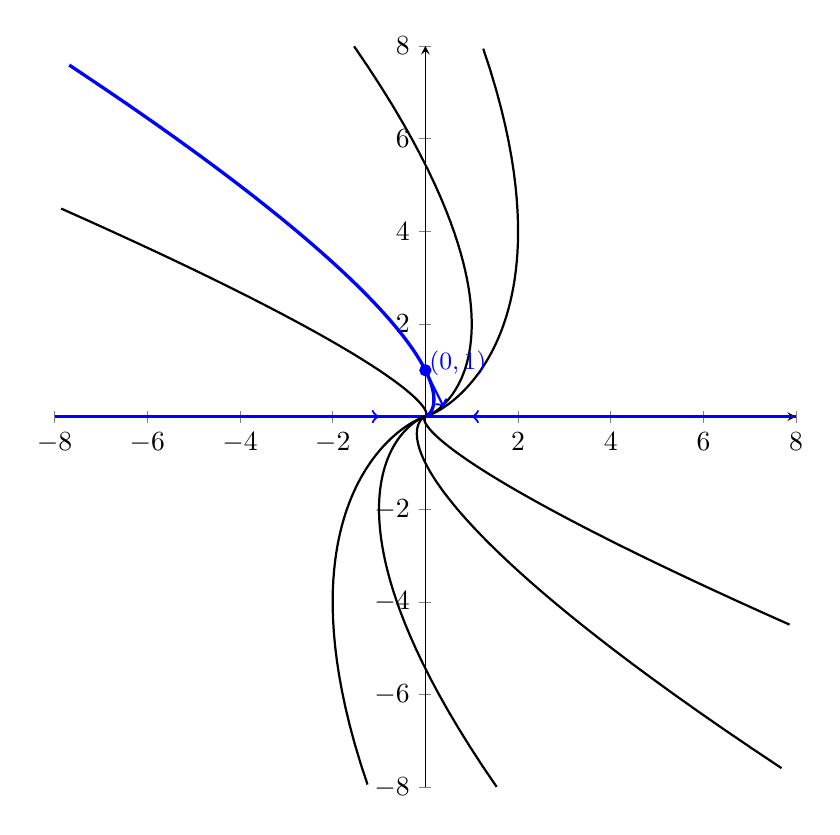
\begin{tikzpicture}
\begin{axis}[
    width=11cm,
    height=11cm,
    axis lines=middle,
    xmin=-8, xmax=8,
    ymin=-8, ymax=8,
    samples=200,
    clip=true,
    restrict x to domain=-8:8,
    restrict y to domain=-8:8
]

% eigenvector line y=0
\addplot[blue, very thick, domain=-8:8] ({x},{0});

% arrows on eigenvector line (toward origin)
\addplot[blue,->, thick] coordinates {(2,0) (1,0)};
\addplot[blue,->, thick] coordinates {(-2,0) (-1,0)};

% sample trajectories
% x = e^{-2t}(c1 + c2 t),   y = c2 e^{-2t}

\addplot[black, thick, variable=\t, domain=-1.8:4]
({exp(-2*\t)*(1 + 2*\t)}, {(2)*exp(-2*\t)});
\addplot[black, thick, variable=\t, domain=-1.8:4]
({exp(-2*\t)*(-1 - 2*\t)}, {(-2)*exp(-2*\t)});

\addplot[black, thick, variable=\t, domain=-1.8:4]
({exp(-2*\t)*(2 + 4*\t)}, {(4)*exp(-2*\t)});
\addplot[black, thick, variable=\t, domain=-1.8:4]
({exp(-2*\t)*(-2 -4*\t)}, {(-4)*exp(-2*\t)});

\addplot[black, thick, variable=\t, domain=-1.8:4]
({exp(-2*\t)*(-1 + 1*\t)}, {(1)*exp(-2*\t)});
\addplot[black, thick, variable=\t, domain=-1.8:4]
({exp(-2*\t)*(1 - 1*\t)}, {(-1)*exp(-2*\t)});

\addplot[black, thick, variable=\t, domain=-1.8:4]
({exp(-2*\t)*(0 - 1*\t)}, {(-1)*exp(-2*\t)});

% highlighted trajectory through (0,1):
% x = t e^{-2t}, y = e^{-2t}
\addplot[only marks, mark=*, mark size=2pt, blue] coordinates {(0,1)};
\node[blue] at (axis cs:0.7,1.15) {\small $(0,1)$};
\addplot[blue, very thick, variable=\t, domain=-1.8:4]
({exp(-2*\t)*(0 + 1*\t)}, {(1)*exp(-2*\t)});

\addplot[blue,->, thick] coordinates {(0,1) (0.4,0.2)};

\end{axis}
\end{tikzpicture}
\caption{Phase portrait of a stable degenerate node. The two linear orbits lie on the \(x\)-axis. The other solutions shear inward to $(0,0)$ in a clockwise orientation.}
\end{figure}
\end{example}

\pagebreak

%%%%%%%%%%%%%%%%%%%%%%%%%%%%%%%%%%%%%%%%%%


\newcommand{\minigrid}{
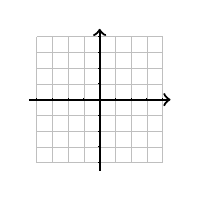
\begin{tikzpicture}[scale=0.2, baseline=-0.6ex]
% grid
\draw[step=1cm, lightgray, very thin] (-4,-4) grid (4,4);

% axes
\draw[->, thick] (-4.5,0) -- (4.5,0);
\draw[->, thick] (0,-4.5) -- (0,4.5);

% tick marks
\foreach \x in {-4,-3,...,4}
    \draw (\x,0.08) -- (\x,-0.08);
\foreach \y in {-4,-3,...,4}
    \draw (0.08,\y) -- (-0.08,\y);
\end{tikzpicture}
}


\section{Summary of All Cases}

\subsection{The Table}
Use the eigenvalues to identify the case. For a repeated nonzero eigenvalue, count the independent eigenvectors to distinguish a star from a degenerate node. Sketch each example on its grid.
\begin{center}

\resizebox{\linewidth}{!}{%
\begin{tabular}{c c c c c}
\hline
\textbf{Type} & \textbf{Major Cases} & \textbf{Sub-cases} & \textbf{Example} & Phase Portrait \\
\hline\\[1mm]
Distinct real & $\lambda_1\neq\lambda_2\in\mathbb{R}$ & \textbf{Node} $\lambda_1 \lambda_2 > 0$ & $\begin{bmatrix}2&0\\0&1\end{bmatrix}$& \minigrid\\[10mm]
 & & \textbf{Saddle}  $\lambda_1 \lambda_2 < 0$& $\begin{bmatrix}2&0\\0&-3\end{bmatrix}$&\minigrid\\[10mm]
 & & \textbf{Line of Equilibria}  $\lambda_1\lambda_2=0$& $\begin{bmatrix}2&1\\4&2\end{bmatrix}$ &\minigrid\\[10mm]
 \hline\\[1mm]
Complex & $\alpha\pm i\beta$ & \textbf{Center} $\alpha =0$ & $\begin{bmatrix}0&-1\\1&0\end{bmatrix}$&\minigrid\\[10mm]
 & & \textbf{Spiral} $\alpha \ne 0$ & $\begin{bmatrix}1&3\\-3&1\end{bmatrix}$&\minigrid\\[10mm]
\hline\\[1mm]
Repeated real & $\lambda_1=\lambda_2\ne0$ & \textbf{Star} & $\begin{bmatrix}6&0\\0&6\end{bmatrix}$&\minigrid\\[10mm]
 & & \textbf{Degenerate} & $\begin{bmatrix}2&-1\\0&2\end{bmatrix}$&\minigrid\\[10mm]
\hline
\end{tabular}}
\end{center}

If both eigenvalues are zero, $A=0$ gives a plane of equilibria. For $A\ne0$, the general solution reduces to $c_1\mathbf{v}+c_2(t\mathbf{v}+\mathbf{w})$. The equilibrium line is spanned by $\mathbf{v}$, and the moving trajectories are straight lines parallel to it.

\subsection{Parameterized Matrices}
\begin{example}[6]{
For the matrix
\[
A=\begin{bmatrix}3&1\\\alpha&1\end{bmatrix},
\]
how does the phase portrait change as $\alpha$ decreases from $0$ to $-2$?
}
The characteristic equation is
\[
0=\det(\lambda I-A)=
\begin{vmatrix}\lambda-3&-1\\-\alpha&\lambda-1\end{vmatrix}
=\lambda^2-4\lambda+3-\alpha.
\]
Its \textbf{discriminant} is $D=16-4(3-\alpha)=4(1+\alpha)$, so the eigenvalues are $\lambda=2\pm\sqrt{1+\alpha}$.
\begin{itemize}
\item At $\alpha=0$, the eigenvalues are $1$ and $3$. Throughout $-1<\alpha\le0$, both are positive and distinct, so the origin is an \textbf{unstable node}.
\item At $\alpha=-1$, the repeated eigenvalue is $2$. This is the matrix from Example 4, with one eigenvector direction, so the origin is an \textbf{unstable degenerate node}.
\item For $-2\le\alpha<-1$, the eigenvalues are nonreal with real part $2$, so the origin is an \textbf{unstable spiral}.
\end{itemize}
The shape changes at $\alpha=-1$ even though the origin stays unstable throughout this interval.
\end{example}
\end{document}
